\begin{center}
\section{System Requirements}
\label{sec:system}
\end{center}

Until this point, the report has primarily focused on research and theoretical designs, but software development is a significant aspect required to prove and analyse the theory. Making the right system design choices is crucial to the success of the project's aims and goals, ensuring that valuable time is not wasted on refactoring and bug fixing. Multiple working computer programs are required to fill all the project needs; therefore, the code should be adaptable and highly interoperable. The programs should utilise state-of-the-art technology to leverage all the benefits to achieve the highest success. Planning and system requirements are crucial, as most IT projects fail because there were not clearly defined requirements\cite{functional_requirements}.

\subsection{Functional Requirements}
\label{sec:requirements}
Functional requirements define what the product(s) should do regarding behaviour and features; achieving these requirements is essential for the project's success. Each requirement can be classified by type, description, and aim in Table\ref{tab:functionalreq}.
\pagebreak

\begin{table}[!ht]
    \centering
    \renewcommand{\arraystretch}{1.2} % Adjust row height for readability
    \begin{tabularx}{\textwidth}{
    |>{\raggedright\arraybackslash}p{3cm}
    |>{\raggedright\arraybackslash}p{1.3cm}
    |>{\raggedright\arraybackslash}p{4cm}
    |>{\raggedright\arraybackslash}X|}
\hline
\multicolumn{1}{|c|}{{\ul \textbf{Name}}} & \multicolumn{1}{c|}{{\ul \textbf{Type}}} & {\ul \textbf{Description}}               & {\ul \textbf{Aim}}                                                                                                          \\ \hline
1.a) Graph Theory                              & Data                                     & Store vertices and edges                    & The program should be able to handle storing any number of vertices and edges in memory as mentioned in Section\ref{graph_data} \\ \hline
1.b) TSP Constraints                           & Logic                                    & Follow the rules of a TSP problem           & The program should not break any of the TSP constraints mentioned in Section\ref{hamiltonian-data}                                                \\ \hline
1.c) Euclidean TSP                             & Logic                                    & Follow the rules of a Euclidean distance    & The program should calculate the Euclidean distance correctly between two vertices                                          \\ \hline
2.a) Facilities for Algorithms                 & Logic                                    & Allow multiple algorithms to be used        & The program should be able to be used for numerous algorithms                                                               \\ \hline
2.b) Benchmarking Algorithm                    & System                                   & Benchmarking of route length and time taken & The program should accurately report and store the results of an algorithm execution                                         \\ \hline
2.c) Algorithm Fairness                        & Perfor-
mance                              & All algorithms should operate at their best & The program should not negatively impact the performance of an algorithm \\ \hline
2.d) Testing Suite                             & System                                   & Allow for multiple different types of tests & The program should be able to run various types of tests with many parameters repetitively and for long periods \\ \hline
3.a) Display TSP Solutions                     & UI/UX                                    & GUI output of the algorithms solutions      & The program should adequately display graphs and Hamiltonian cycles                                                         \\ \hline
4.a) Collect Test Data                         & Data                                     & Collect multiple instances of test data     & The program should use secondary storage, a proper text-based formatting system                                             \\ \hline
4.b) Analysis Test Data                        & System                                   & Produce statistics and graphs               & The program should provide data analysis on the collected data to produce meaningful statistical insight                    \\ \hline
5.a) Unit Test                                 & System                                   & Adequately unit test code base              & The program should have unit test coverage of the core shared library codebase, focusing on systems used by every component \\ \hline

    \end{tabularx}
    \caption{Functional Requirements}
    \label{tab:functionalreq}
\end{table}
\pagebreak

\subsection{Non-Functional Requirements}

Non-functional requirements define the level of quality the product(s) should have in terms of behaviour and features; achieving these requirements is not essential for the project's success but would be beneficial. Each requirement can be classified by its aim and type in a table.
\vspace{0.4cm}
\begin{table}[!ht]
    \centering
    \renewcommand{\arraystretch}{1.2} % Adjust row height for readability
    \begin{tabularx}{\textwidth}{|X|p{3cm}|}
    \hline
{\ul \textbf{Aim}}                                                                         & {\ul \textbf{Type}} \\ \hline
The user should be able to select the type of algorithm they want easily                   & Usability           \\ \hline
The program should never fail or crash                                                     & Reliability         \\ \hline
The program should be responsive and utilise all computing power                           & Performance         \\ \hline
The program should be adaptable and fill the needs of each executable                      & Scalability         \\ \hline
The GUI should be easy to read for all users, e.g. inclusive of those with colour blindness & Usability           \\ \hline
    \end{tabularx}
    \caption{Non-Functional Requirements}
    \label{tab:nonfunctionalreq}
\end{table}

\subsection{C++}
\label{sec:c++}
C++ is a low-level programming language first created in 1985 by Bjarne Stroustrup\cite{stroustrup2013cpp}. It is widely used in algorithmic research and industry due to its high performance and low-level capabilities. In this project, C++ was selected as the primary language due to prior experience and previous personal projects involving the language. MSVC\cite{visualstudio_cpp} compiler was used as it integrates seamlessly with Visual Studio and C++20\cite{cppreference_cpp20} for it is the most modern long-term support(LTS) version.

C++ has no built-in memory management and relies on the programmer to handle allocation and deletion. This removes the overhead of an automatic memory management system but can lead to data corruption or memory violations. The benefit of allowing the programmer to decide is the ability to use either stack vs heap memory.
\begin{itemize}
    \item Stack: Faster but limited by size and must be known at compile time
    \item Heap: Unlimited size and can be dynamically allocated, but slower as it requires OS system call and uses a pointer to access.
\end{itemize}

Accessing memory is a leading cause of slow performance times due to cache misses \cite{drepper2007memory}. C++ has low-level calls that are unique to low-level languages, allowing for direct manipulation of computer memory. This allows for logical memory tricks and greater control over memory to accommodate each system's architecture\cite{memorymanagement}. Both must be used when programming in C++, but stack memory is favourable in most situations.

Object-Oriented Programming(OOP) has become the standard programming paradigm for most use cases. OOP is dynamic as encapsulation and polymorphic properties can be applied to most problems. The abstract nature and use of Creational Patterns lend OOP well to this project for initiating multiple algorithms.  

\subsubsection{API \& Interfaces}
\label{sec:API}

To satisfy the multiple functional requirements(Table\ref{tab:functionalreq}), various computer programs(executables) will need to be developed to achieve each of the different requirements. Each program will require the same features and data, so to avoid bugs and repetitive code; core functionality is placed in a library. There are two types of libraries in C++:

\begin{itemize}
    \item Static Library: Library code is added to the source code and compiled at compile time
    \item Dynamic Library: Library code is compiled into a DLL and linked at run-time
\end{itemize}

The benefits and differences depend on a few factors, but the static library was preferred due to template metaprogramming(Section\ref{template}). However, both remove the dependency of an owner, and a static library acts as the project's base. To ensure practical software development, it is still essential to understand how the library functions and interacts with each program; this is achieved by following standard Design Patterns, APIs, and Interfaces.

As seen in Section\ref{lit}, several stages and optimisations can be applied to create an overall heuristic, including tour constructors, tour optimisers, partitioning systems, and caching modes. To construct any number of combinations by hand would be infeasible, so a Creational Pattern in OOP, called a Builder\cite{refactoringGuruBuilder}, is used like a cookie cutter for each option. The idea is to have a single Builder class that utilises composition to construct the algorithm for the possibilities it provides. This requires interfaces for the builder class to call upon its objects.

\begin{figure}[H]
    \centering
    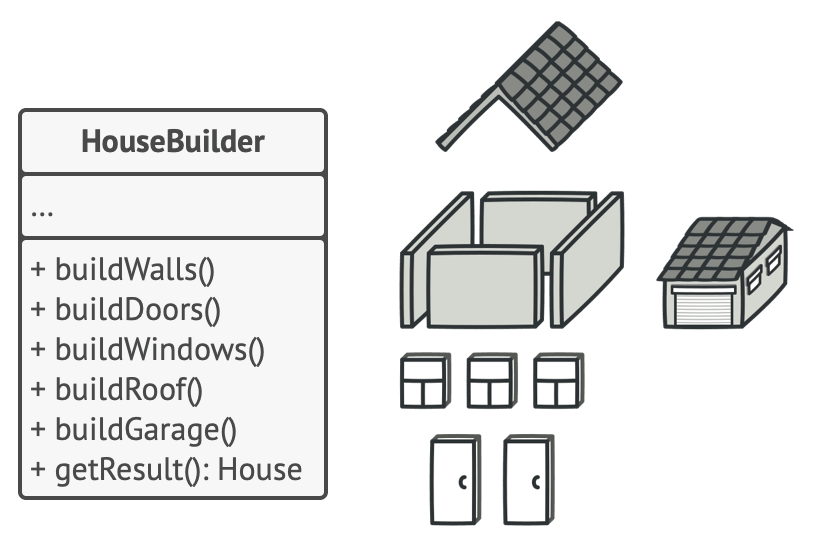
\includegraphics[width=0.5\textwidth]{sections/image/Builder.png}
    \caption{Builder Pattern}
    \cite{refactoringGuruBuilder}
\end{figure}

Interfaces are public abstract classes that utilise the polymorphic nature. Abstract classes cannot exist as objects due to being incomplete classes, but they can be inherited by child classes to gain their properties. This ensures that each built object has the correct interface for immutability within the larger system.

To ensure the user(programmer) does not interact with the library incorrectly, APIs are used to limit the control they have over the underlying data. API's also help programmers more easily understand what the code is doing and what the original creator had in mind. APIs are heavily relied upon for communication between the library and each executable.

\subsubsection{Template Metaprogramming}
\label{template}

Template Metaprogramming(TMP) is an additional step in the C++ compiler that introduces compile-time polymorphism by utilising template functions\cite{vandevoorde2002c++}. It allows a single template function to have infinite copies of itself without requiring additional code. Template functions require a template variable, which takes the values of data types, functions, or constant values. At compile time, the template function variables are instantiated in the template functions to create inlined generic source code.

\begin{lstlisting}[caption={Template Code}, label={fig:template},numbers=left]
template<typename var>
void foo(var a) {
    std::cout << "value : " <<  a << "\n";
}

/*
What the compiler would generate:

void foo<int>(int a) {
    std::cout << "value : " <<  a << "\n";
}

void foo<std::string>(std::string a) {
    std::cout << "value : " <<  a << "\n";
}
*/

template<int var>
class goo {
public:
    static void bar() {
        std::cout << "value : " << std::to_string(var) << "\n";
    }
};

/*
What the compiler would generate

static void goo<5>::bar() {
    std::cout << "value : " << std::to_string(5) << "\n";
}
*/

int main()
{
    foo<int>(10);                 // print "value : 10"
    foo<std::string>("hello");  // print "value : hello"
    
    goo<5>::bar();                // print "value : 5"
}
\end{lstlisting}

In the example, Listing\ref{fig:template}, $foo()$ is a template function, and var is a template function variable. In the $main()$ function, foo is instantiated with the data types $int$ and $string$, and then arguments of those types are passed. The program compiles and runs as expected, with the $foo<int>()$ and $foo<string>()$ functions being generated before compile time, as represented by the code in the comment(Line 9). Classes can also have templates, which can define member fields and functions(Listing\ref{fig:templateAdv}).

\begin{lstlisting}[caption={Advance Template Code}, label={fig:templateAdv},numbers=left]
class abstract {                    // Pure abstract class 
    virtual void foo() = 0;
};

class child : public abstract {    // Abstract child class
    void foo() override {
        std::cout << "real function";
    }
};

template<typename T>
class real {
    static_assert(std::is_base_of<abstract, T>::value, "T must derive from abstract");
    
    T var;  // Compile-Time Polymorphism: In-line real class without V-Table
};

int main() {
    real<child> b;    // Abstract class on the stack
}
\end{lstlisting}

Metaprogramming has its roots in compiler development but is heavily applied in performance optimisation code. This is because a constant expression can be evaluated at compile time, leading to the removal(inlining) of branching and expression evaluation. Much like its name, compile-time polymorphism, metaprogramming\cite{abrahams2004c++} can mimic OOP polymorphism at compile time(Listing\ref{fig:templateAdv}). This is faster than normal polymorphism, as it eliminates the V-Table, which determines which child virtual function to invoke. Calling the V-Table incurs a constant time slowdown, which is undesirable when performance is a concern and the number of calls varies between TSP algorithms.

\begin{figure}[!ht]
    \centering
    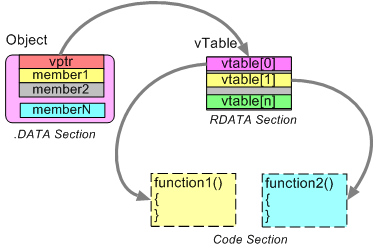
\includegraphics[width=0.7\textwidth]{sections/image/vptr-vtable-vfunctions.png}
    \caption{C++ V-Table}
    \cite{refactoringGuruBuilder}
\end{figure}

Another performance benefit of TMP is compile instantiation. Many data types must be placed on the heap due to their dynamic size, which incurs a performance hit with each call. As TMP instantiates classes with the type in place at compile time, it can allocate a static size on the stack for abstract child classes, thereby avoiding any performance hit(Listing\ref{fig:templateAdv}). 

As this project is heavily performance-focused, fairness is necessary; not using templates would be a mistake. Compile-time polymorphism enables builder classes with constant slowdowns to behave like a monolithic class, allowing in-line and optimisation of function calls. Templates have their disadvantages, including steep learning curves, reduced flexibility, additional complexity, difficult to debug, long compilation times, and memory usage issues; however, these are negligible for the scale and scope of this project.

\subsubsection{QT6}

QT\cite{qt6} is a cross-platform GUI library for creating graphical applications natively on all operating systems and embedded hardware. It is written in C++ but can also be developed with Python. QT6 is the most modern iteration, having undergone 29 years of development and featuring an open-source license, making it a go-to choice for research and non-profit developers. The needs of this project do not necessitate a wide use of graphical features, which is why choosing QT6, with its extensive catalogue of tutorials, was ideal.

\begin{figure}[!ht]
    \centering
    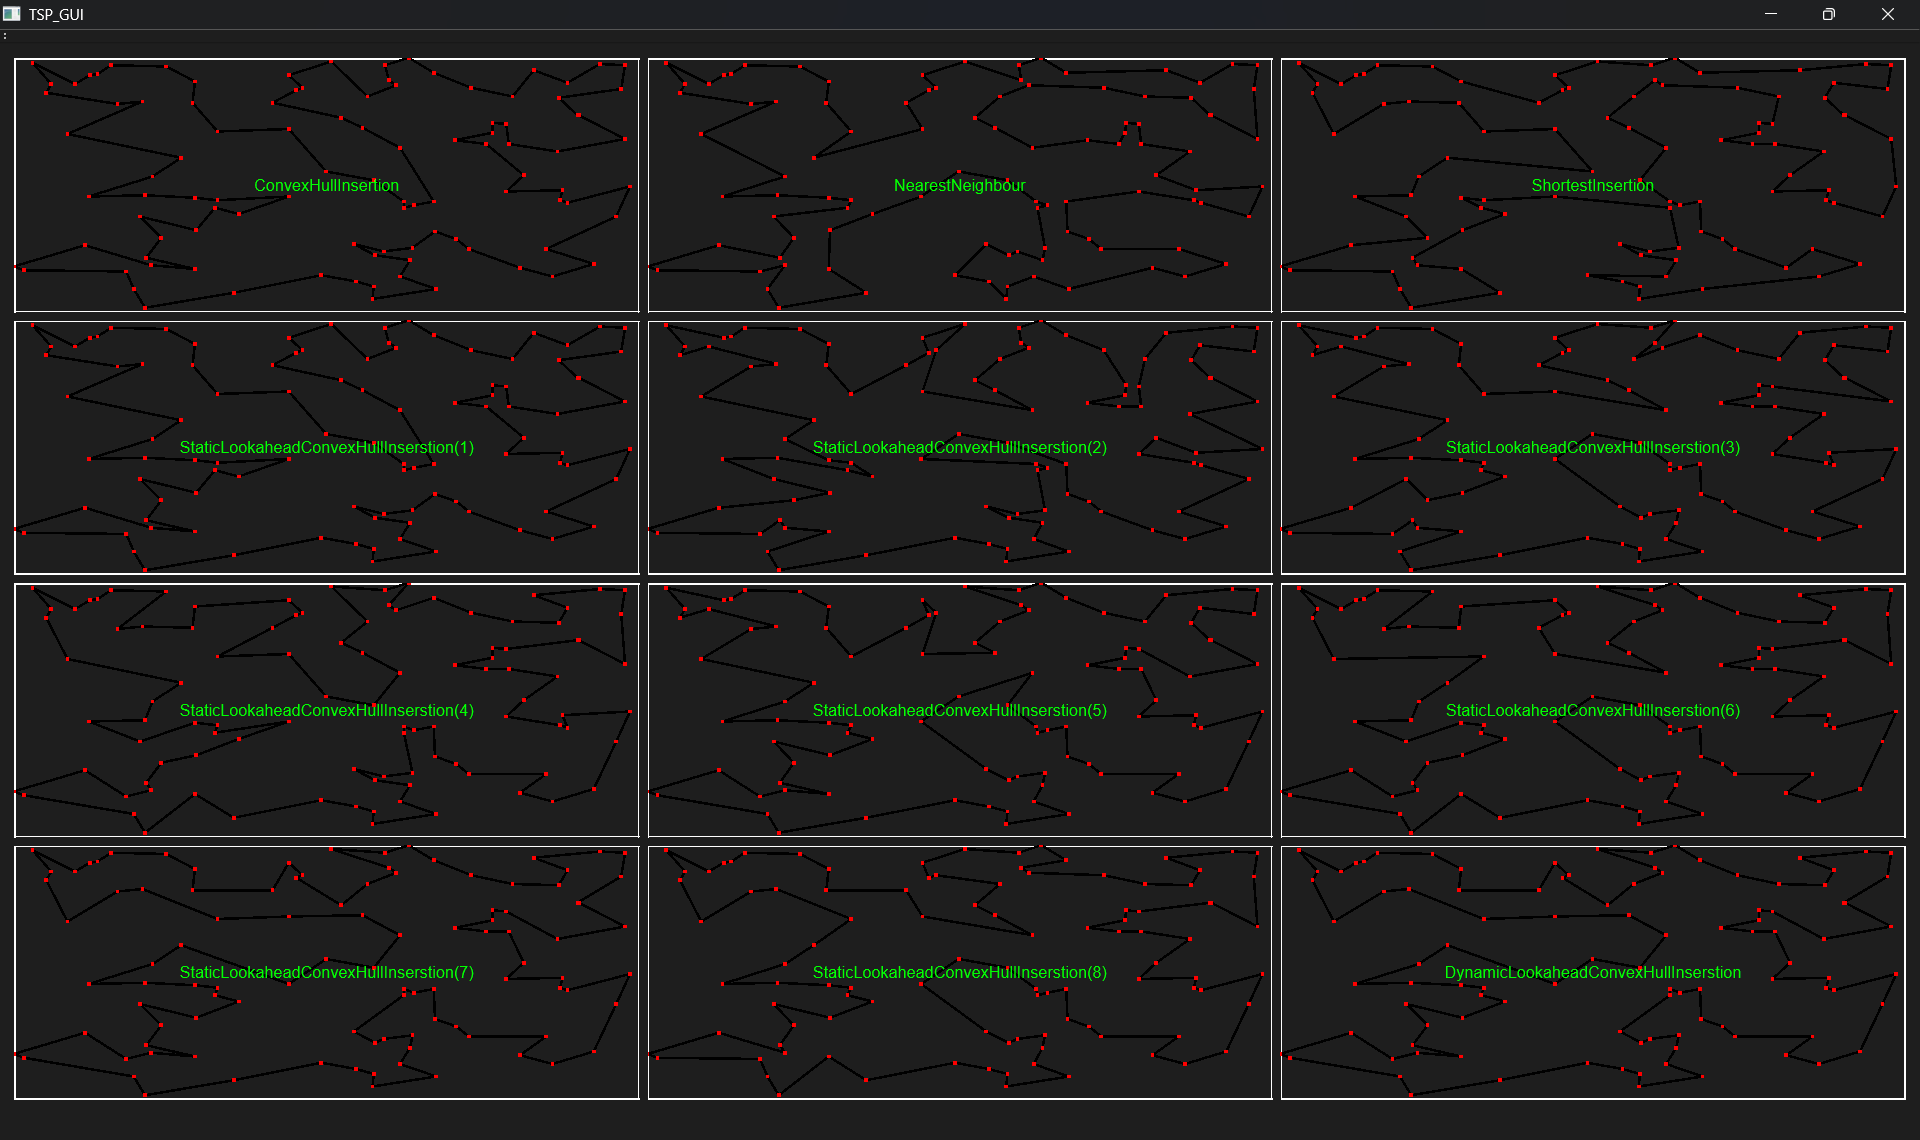
\includegraphics[width=\textwidth]{sections/image/Result.png}
    \caption{Example: QT6 Application GUI}
\end{figure}

\subsubsection{C++ Libraries}
\label{cpplibrar}
Libraries are valuable resources for ontaining a pre-made solution to complex functionality that developers widely encounter. However, when C++ was being developed, library support and development were not as prolific as modern languages. For this project, the libxlsxwriter library\cite {libxlsxwriter} helped generate Excel files. GNU Scientific Library\cite{gsl} was used for the gradient descent function in optimising the dynamic look-ahead arguments. 

\subsection{Hardware}

Hardware is a crucial factor in testing NP-hard problems; from tiny microcontrollers to massive supercomputers, the amount of available computing power determines the problem size and the type of algorithm that can be used. The project was completed using a home desktop PC running Windows 11, equipped with an Intel i9-13900 processor and 32GB of RAM. 

\subsubsection{Consistency}

For the fair testing of algorithms(Section\ref{method}), physical and external factors need to be controlled as a control variable to prevent bias. Physical factors comprise of power draw to thermal temperatures, while external factors include background tasks and execution mode. With no funding or external resources, controlling many of the variables was hindered.

Thermal temperatures of the CPU constitute the most significant downfall; excessive heat can trigger thermal throttling, reducing performance. Managing thermal temperatures with effective cooling systems and maintaining a consistent ambient temperature was not possible with the available setup. Therefore, overclocking the CPU was disabled to maintain a stable clock rate for extended periods.

When compiling the program, the identical execution flags and release mode should be constant. Tests should not be run quickly after boot or with background tasks running, as these may consume CPU time.

\subsubsection{Multi-Threading}

To fulfil the non-functional requirements(Table\ref{tab:nonfunctionalreq}) and reduce the time required to gather all the data, tests are run in parallel. Each process also uses asynchronous timeout calls to prevent tests from running indefinitely. Therefore, a multi-core processor is a requirement for achieving stable performance.

\subsubsection{Memory}

The Travelling Salesman Problem and look-ahead design can consume a significant amount of memory if the problem is sufficiently large. With modern hardware storing GB of RAM and MB of cache, the space capacity is not likely to be a limiting factor. However, the constant reading and writing of memory can hinder performance; therefore, quicker RAM is favourable.
